\chapter{Research questions} \label{chapter:research}
In this chapter, the research questions for the thesis are formulated. What research method will be used, and how the questions be validated.

\section{Context}
This thesis revolves around change detection and visualising the comparison between two consequent versions of the application under test. The result is an external application that connects to OrientDB and calculates and shows the model comparison. Figure \ref{fig:components-overview} shows the different components involved. The \textit{New Analysis Website} component is the component that is created. Section \ref{sec:components-explained} explained the different components in more detail.

The external application is built as a separate application next to the \testar application. The code that Pastor Ricós created (Section \ref{sec:state-model-difference}) and Mulders (Section \ref{inferred-model}) is used as a starting point for the external application. 

\begingroup
\captionsetup{type=figure}
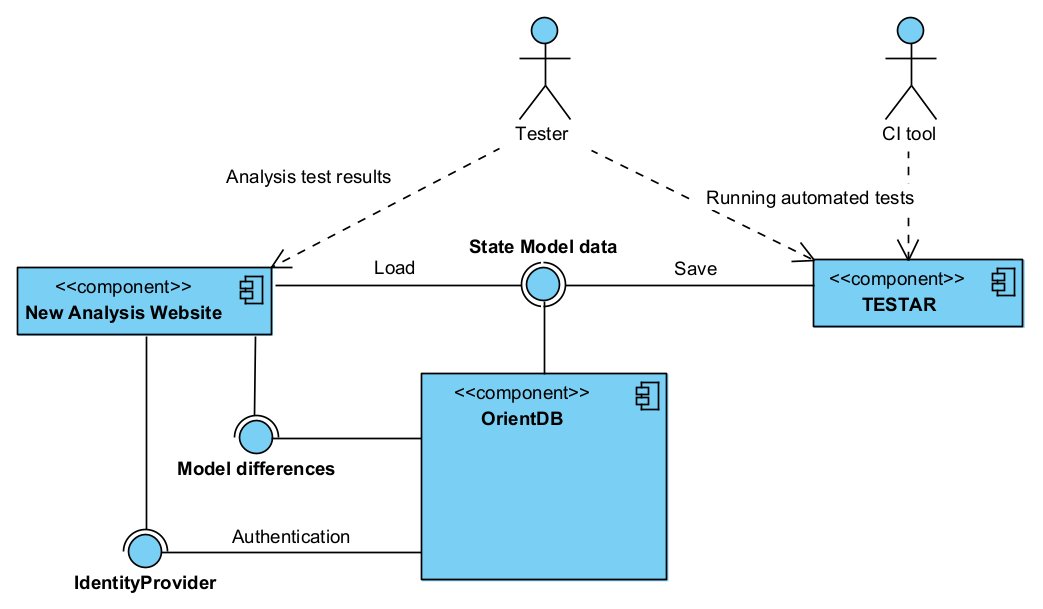
\includegraphics[scale=0.4]{images/3-UML-high-level.png}
\captionof{figure}{Components overview (UML 2.0)}\label{fig:components-overview}
\endgroup

Because change detection is the subject of this graduation assignment, it is assumed that the inferred model generator will generate useful models for change detection. Although the inferred model generator is out-of-scope, it is not ruled out that changes are necessary.

\section{Research questions} \label{research-questions}
% Note: the question are defined as variables in ..\main.text so they can be used throughout the thesis without having them to copy-past and keep them up-to-date manually. 

The main research question is:

\textbf{\rqMainQuestion}

The main research question is divide into three sub questions:

\begin{questions}
    \item \rqApplicationOutsideTestar \label{rq:application-outside-testar}
    \item \rqHowMakingChangeDetectionAlgorithm \label{rq:how-making-change-detection-algorithm}
    \item \rqHowToVisualiseResult \label{rq:how-to-visualise-result}
\end{questions}

In the next sections the research questions are explained in more detail.

\subsection{\ref{rq:application-outside-testar} \rqApplicationOutsideTestar}

The outcome of \ref{rq:application-outside-testar} is a website that the testers can use to analyse the test results and execute the change detection algorithm. The current analysis website is embedded in the \testar tool. Since \testar can run inside a container during a continuous deployment \cite{thesisSlomp}. Even though testers do not need \testar to run tests on the GUI, they need to install \testar onto their computers to view the analysis website. 

Additional work needs to be done to create the new analysis website. Industrial standards need to be implemented, including but not limited to web security, authentication to the web server, providing easy navigation and switching of orientDB databases. 

The approach to creating the application outside of \testar will be conducted iteratively and incrementally in collaboration with the supervisors and F-Secure. During each weekly meeting, updates will be given, and feedback will be incorporated as soon as possible. 

\subsection{\ref{rq:how-making-change-detection-algorithm} \rqHowMakingChangeDetectionAlgorithm}

The outcome of \ref{rq:how-making-change-detection-algorithm} is an implementation of change detection on the abstract layer of two versions of the GUI. The change detection algorithm will not be executed on the concrete layer since that layer can contain a 
Especially since every change in the widget tree, like the button background, triggers a new state in the concrete layer. 

The technical aspects of the change detection algorithm are validated with an experimental application. In a later stage, the algorithm is validated with research question \ref{rq:how-to-visualise-result} since it is hard to validate an algorithm without seeing the results. 

\subsection{\ref{rq:how-to-visualise-result} \rqHowToVisualiseResult}

After the change detection algorithm, the output must be displayed to the user. with \ref{rq:how-to-visualise-result} an research is conducted how to. Besides the research, the actual visualisation requirements will be discussed with the \testar stakeholders.